\documentclass[12pt]{article}

\usepackage{amssymb,amsmath,amsthm}
\usepackage{graphicx}
\usepackage{pgfplotstable,booktabs,longtable} % Package for including figures
%\usepackage{psfrag,color}

\title{Homework 4 \protect \\(Math/CS 471)}

\author{Elijah Perez \protect \newline \\ Natalie Chang}


\date{\vfill 10/11/2020}   



\begin{document}
	\maketitle
	\pagebreak
	
	\section{Introduction}
    This report explores the finite difference methods for calculating partial derivatives. The functions that we are taking the derivative of require application of the chain rule to find the derivatives. We will find the error in our estimated for the derivative using an integration error method. The specific equations that will be differentiated can be found in the Equations section, the results can be found in the Results section, and any final remarks can be found in the Conclusion section.
	
	\section{Equations}
	The equations that are being differentiated are:
	\begin{equation}
		u_1(r,s)=[(4s^2+r^2)sin(s+r)]^2+[(3s+r^2)cos(s+r)]^2
	\end{equation}
	\begin{equation}
		u_2(r,s)=[r^2+2s]^2+[3r+s^2]^2
	\end{equation}
	\begin{equation}
		u_3(r,s)=r^2+s^2 
	\end{equation}	
	Note: These functions are defined as $u(x,y)=x^2+y^2$ with x and y being defined through r and s. This has the nice result that $u_{xx}+u_{yy}=4$. This is something that can be used to see if the approximate derivatives make sense.
	
	\section{Results}
	Below are graphs showing the error of the derivatives of u as well as the domain plots:
	
		\begin{figure}
			\centering
			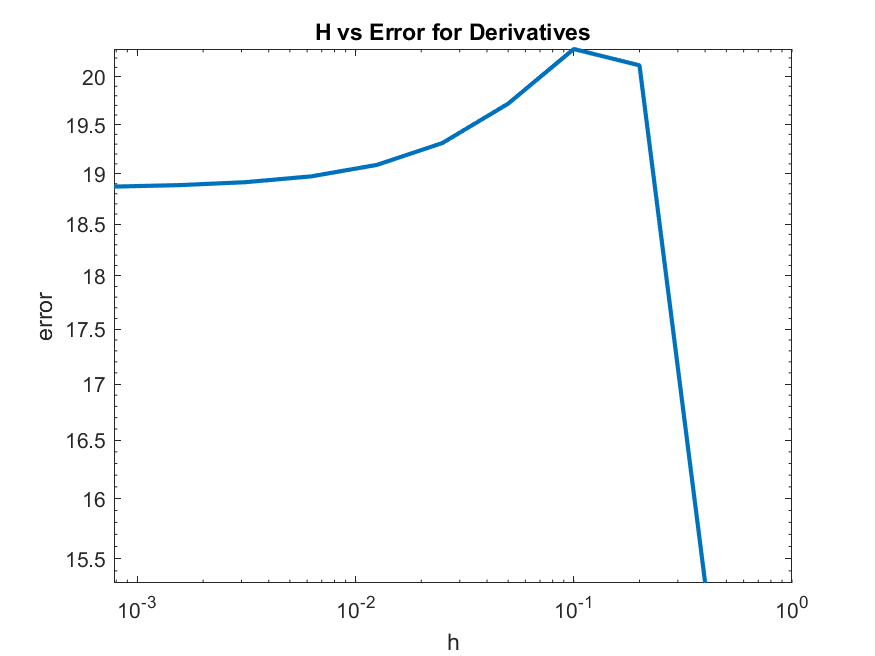
\includegraphics[width=100mm,height=60mm]{error1.png}
			\caption{error for derivatives of $u_1$}
		\end{figure}
		\vspace{1in}
		\begin{figure}
			\centering
			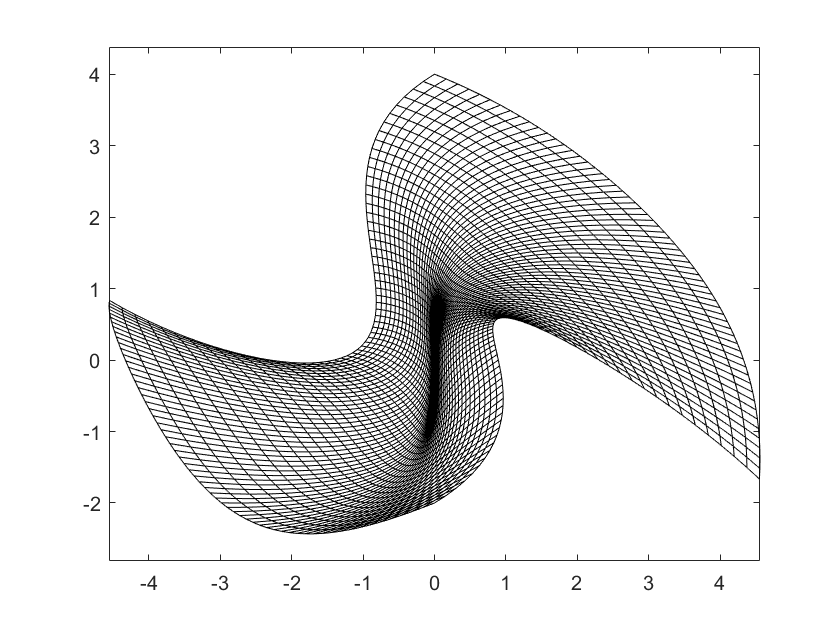
\includegraphics[width=100mm,height=60mm]{function1.png}
			\caption{Domain of $u_1$}
		\end{figure}
		\begin{figure}
			\centering
			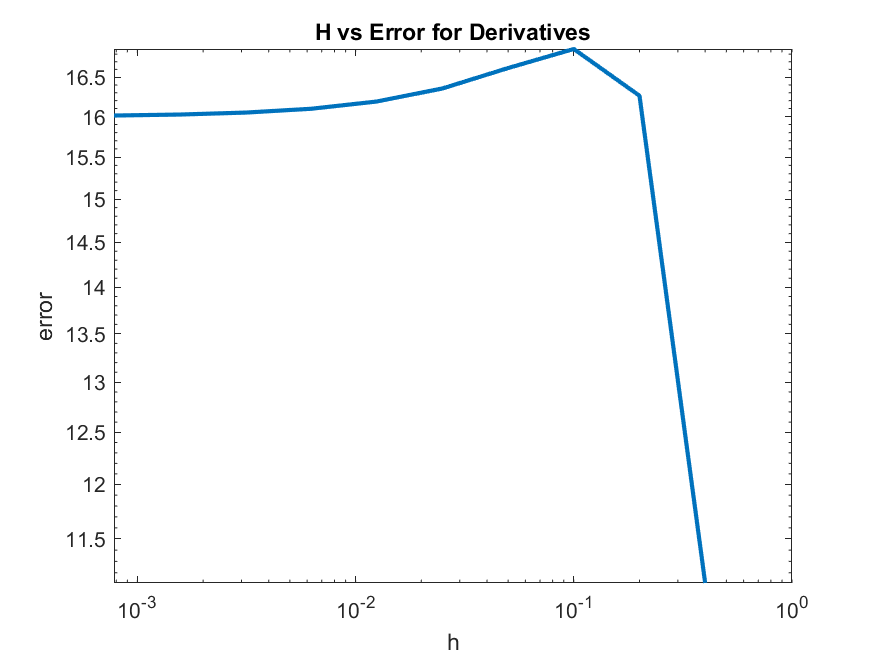
\includegraphics[width=100mm,height=60mm]{error2.png}
			\caption{error for derivatives $u_{2}$}
		\end{figure}
		
	    \begin{figure}
	    	\centering
	    	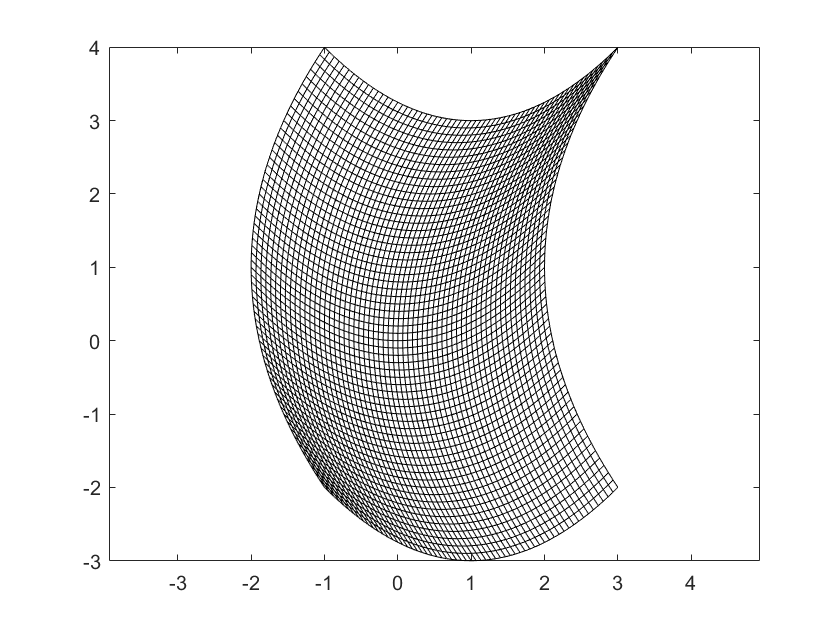
\includegraphics[width=100mm,height=60mm]{function2.png}
	    	\caption{Domain of $u_2$}
	    \end{figure}
    	\begin{figure}
    		\centering
    		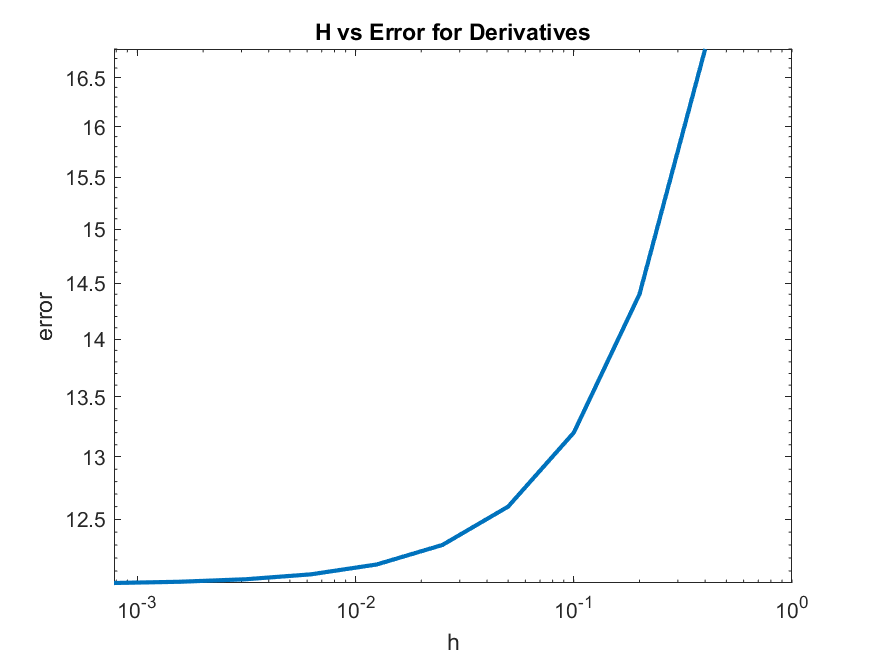
\includegraphics[width=100mm,height=60mm]{error3.png}
    		\caption{error for derivatives of $u_3$}
    	\end{figure}
        \begin{figure}
        	\centering
        	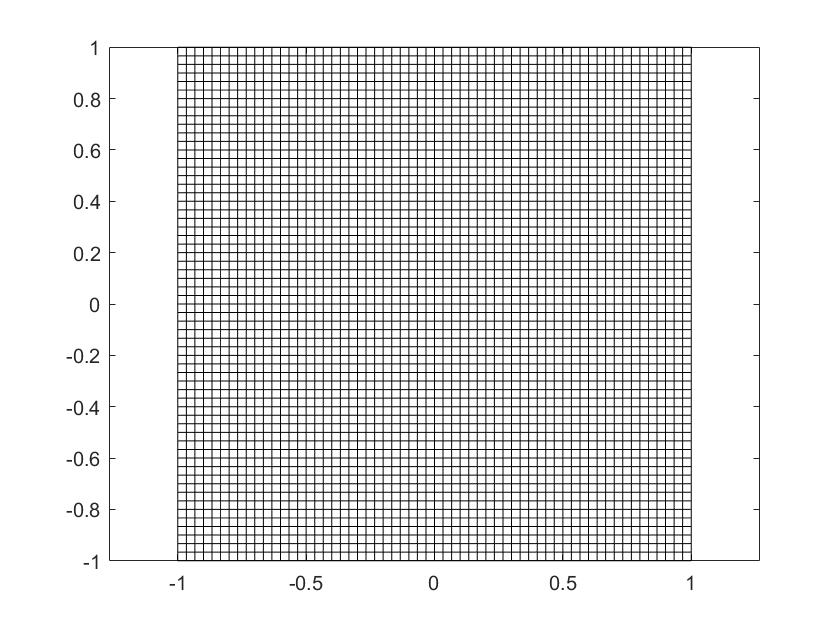
\includegraphics[width=100mm,height=60mm]{function3.png}
        	\caption{Domain of $u_3$}
        \end{figure}
        \begin{figure}
        	\centering
        	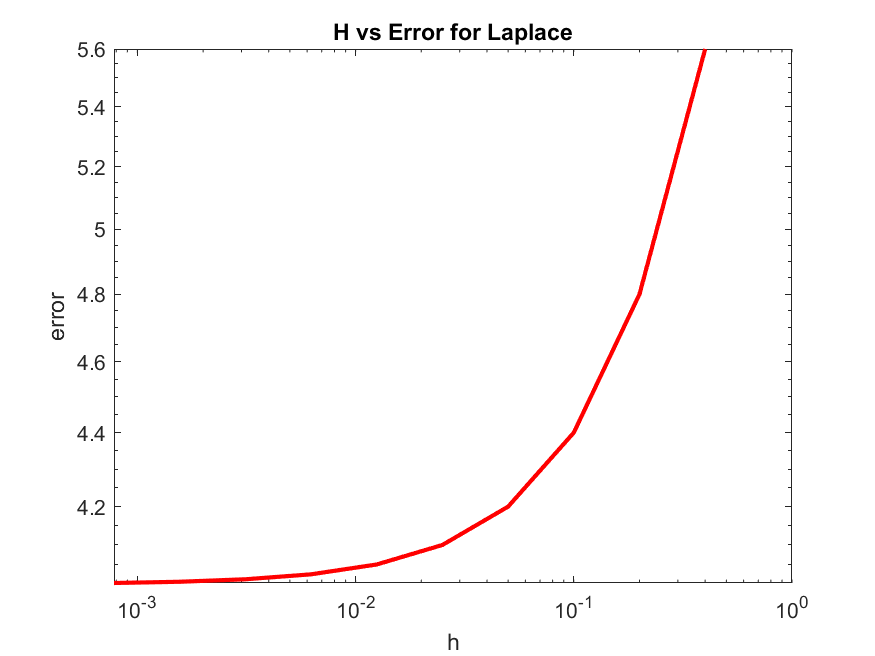
\includegraphics[width=100mm,height=60mm]{errorLaplace3.png}
        	\caption{error of $\Delta u_3$}
        \end{figure}
        \pagebreak
    	
    	\section{Conclusion}
    	The main findings from this experiment is that the method used to find estimates for the partial derivatives is accurate. This can be confirmed by comparing the analytic solution to $\Delta u$, which is always 4, to the solution calculated by the program. \\ When looking at the error for the derivatives of $u_3$ as well as $\Delta u_3$ we see an expected behavior. As h decreases so does the error. We only see this behavior in the error for $u_1$ and $u_2$ for small h values. The unexpected decrease in error for larger h values may be due to numerical errors such as cancellation. Another thing we can see is that as the function becomes more complicated, the starting point for the error is higher. This can be seen in the error for $u_1$ which is the most complex function versus the error for $u_3$ which is the simplest. The errors start at 19 (Figure 1) and 12 (Figure 5) respectively. \\ Analyzing the error of $\Delta u_3$ we see that it is the smallest error by far (Figure 7). This is possibly due to the fact that the true value of $\Delta u_3$ is just 4. This leaves little room for computational errors when calculating the overall error via the integration method. This experiment should be repeated with other functions to confirm these results. 

\end{document}  
